%%%% This section is in essense a restructured and slightly modified chapter of the CDR
%%%% on same subject. Giles was reportedly not available to write new stuff, and it's not clear if it's
%%%% really needed at this point   ---mxp--- 

\section{The Data Acquisition (DAQ) System and Monitoring}
\label{sec:daq}

\subsection{Overview}

The scope of the DAQ and monitoring includes the design, procurement, fabrication, testing, delivery and installation. It is required to:
\begin{itemize}
\item collect data with a very high uptime (the goal is $>99\%$)

\item collect beam neutrino, atmospheric neutrino and proton  decay candidates (generally all interactions
with total energy deposition above about 100\,MeV) with a high resolution (smart or no   zero-suppression) with no dead-time.

\item have the capability to collect interactions with total energy  below $100$\,MeV with some
 low amount of zero-suppression loss.

\item have the ability to trigger at the time of the beam pulses,  irrespective of how little energy is deposited in the detector.

\item collect data with the most favorable zero-suppression possible over a  period of >10\,s (supernova trigger)

\item assemble data from sub-detectors into a unified  event for offline analysis.
\item provide access to the shift operator and others to control and   monitor the data collection and detector status, view online
  histograms and monitor (and provide for offline use) historical  status of measured detector parameters. 

\end{itemize}
%The design presented here   AH: this sounded too bold, somehow.
This section outlines a conceptual design intended to meet the required performance for the DAQ
for the DUNE far detector. 


\subsection{The DAQ Architecture}

To reduce downtime considerably (i.e. time periods when none of the DUNE modules are collecting data, which impacts supernova detection)
and to allow the DAQ technology in the different 10-kt sections to be entirely different if desired, the DUNE DAQ employs a decoupled 
design. The synchronization, triggering, data collection and run-state in the different 10-kt modules are completely independent in real time and
are only coupled by processes running asynchronously (in the same fashion as a batch queue) in the hour or so after data collection.
This allows one portion of the detector module to be restarted without interrupting
data collection in the others.

The layout of the DAQ is shown schematically in
Figure~\ref{fig:fddaqblock}.  To collect full detail of the
most important events (deadtimeless detection of all those with energy
deposition of 100\,MeV and above), while avoiding tricky communication
to flag neighboring channels to those that have large hits, a model is used
in which the digitised data are collected twice from the initial data
storage that is associatated with each peice of hardware. 

%%%%%%%%%%%%%%%%%%%%%%%%%%%%%%%%%%%%%%
% GB - I can't think of anything better, unless we expand this section
% a lot, which whould give it too much emphasis.  Ideally we DO want
% to flag neighbouring channels to those with big hits, but it is
% difficult because it would entail a big complicated network of
% comunications between all the boards which is very tricky.
%\fixme{Previous sentence not clear: you want to flag channels that have large hits and NOT flagneighboring channels?  What's the `tricky communication'?}

The first collection supplies a centralized software-based trigger farm continuously with
zero-suppressed information (a threshold on each channel detects hits above the noise level;
this causes the ADC samples to be kept in a time window around the hit).  
The second collection reads the full data at the times and in the regions %of interest that have been 
selected by the trigger. This is similar to the multi-level triggering in a collider experiment,
but with only one level of triggering. The software trigger farm also
records the continuous stream of zero-suppressed hits in an archival
ring buffer on disk to allow later analysis of supernova candidates.

\begin{figure}[h!]
	\centering
	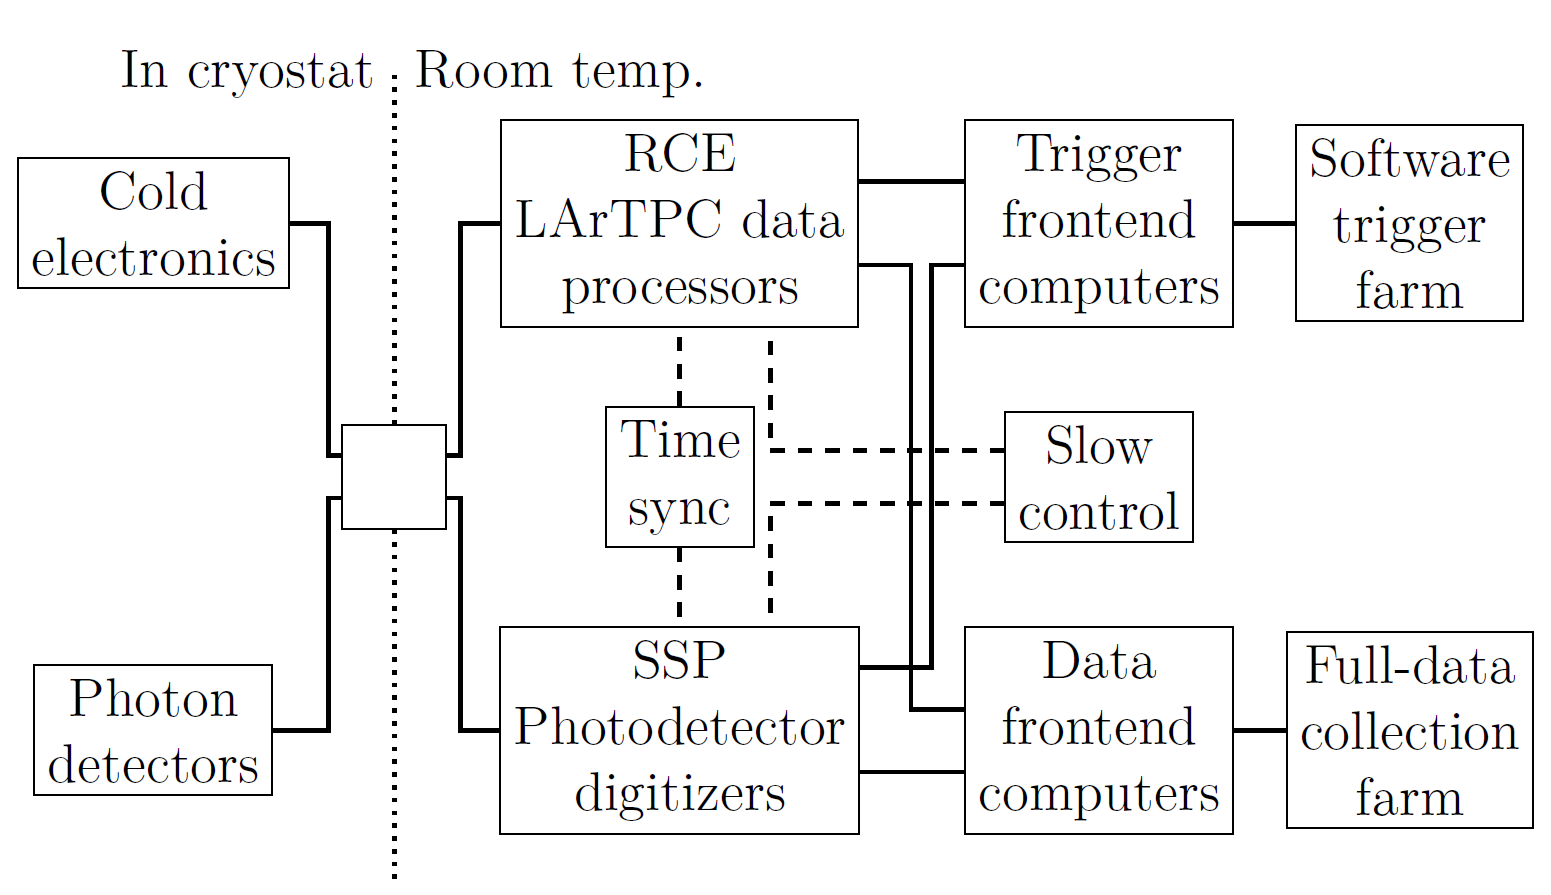
\includegraphics[width=0.8\textwidth]{daq-block-diagram.png}
	\caption{Block diagram layout of the main components of the DAQ subsystem.}
	\label{fig:fddaqblock}
\end{figure}


\subsection{Hardware and Software Components of the DAQ}
\subsubsection{LArTPC detector readout}

The LArTPC signals are digitized in the cold in a continuous flash-ADC stream at 2\,MHz, (not zero-suppressed)
and serialized on 12,000 high-speed links per 10-kt module that exit the cryostat.

The data are received by LArTPC data processors called RCEs (Reconfigurable
Computing Elements) housed in industry-standard aTCA crates on COB (cluster-on-board)
motherboards that are designed at SLAC for a wide range of applications.  The RCEs are part of a
network of field programmable gate arrays (FPGAs) that buffer the full raw data,
zero-suppress it for passing to the trigger and accept requests for
data-fetching from the trigger.  The FPGAs in the RCEs are from the
Xilinx Zynq family and contain a full Linux processor system on the
chip.  They facilitate the high-speed data transfer from firmware into
DRAM memory that is accessible from Linux.  A fast data-transfer
network using the Ethernet protocol is used on the COBs and in the
aTCA crates to allow for development of more sophisticated zero-suppression algorithms
for improved supernova acquisition.

\subsubsection{Photon detector readout}

As described in~\ref{sec:pd}, the Photon Detector readout  is performed by the ``SSP'' module.
 The additional buffering required for the separate trigger and data collection paths
is implemented in the SSP frontend computers.

\subsubsection{Computer farm}
Both the LArTPC and photon detector data are
received in commodity Linux computers, with no deadtime, from where
the data are routed to the trigger and full-data collection farms of
computers.  Although the front-end computers are logically distinct as
shown in Figure~\ref{fig:fddaqblock}, one physical computer is
sufficient for all the processes for each rack of APA readout
electronics. 

\subsubsection{artDAQ software toolkit}

(from Fermilab) supplies the real-time
data collection functionality (buffering, matching event parts,
synchronization, inter-process communication, etc.) in a modern
design that facilitates the efficient use of multicore commodity
computers running on the Linux computer farms.  The multi-core
functionality is crucial in the high data-rate environment on DUNE.  
The detector-specific
code is supplied by DUNE groups (this is centered in the UK), along
with detector-specific triggering (also UK).  The architecture
provided by artDAQ can be tailored for each experiment and is entirely
suitable for the ``collect-twice'' architecture envisioned for DUNE.

\subsubsection{ Run Control and Slow Control software framework}

manages the
control, status display and status archival of the experiment.  It is
based on the ICECube design.  This
exploits a combination of readily available, well-supported packages
[message passing (zeroMQ), a web-framework (Django), databases (postgres)] 
to give the shift operator a unified view of the status
of the running experiment, and views of the monitoring data including
customized views and historical views.  The database of slow-control
measurements is exported to the host lab to give access for offline
programs.

\subsubsection{Timing system}
To acomplish the software-based deadtimeless data
acquisition in DUNE, it is necessary to synchronize the clock across
all readout boards.  This is accomplished in two stages, the main
cavern-wide distribution uses the design from the NO$\nu$A experiments
which distributes a 64-MHz clock, synchronization pulses and
cable-delay correction on RJ45 cables.  The overall clock is
synchronized using a GPS receiver and transferred from the surface
over optical fiber.  The synchronization is transferred from the COBs
to the electronics in the cryostat over the same cabling as provides
the data links.

\subsubsection{Calibration system}
At the time of writing, the calibration system is in the R\&D stage and its design will
evolve as the experiment is being built. Very roughly, there will be three stages:
\begin{enumerate}
\item Pedestal and charge-injection pulser events are used to calibrate and
remove drifting of the individual electronic channel responses.

\item External UV lasers are directed into the cryostat through glass-tube
ports, and swivelling mirrors select the trajectories of the beams
through the cryostat to provide calibration of the field
non-uniformities and attenuation.

\item Cosmic-ray muons are used for the determination of the energy scale and for calibration
cross-checks.
\end{enumerate}



\subsection{The Time Sequence}
\begin{figure}[h!]
	\centering
	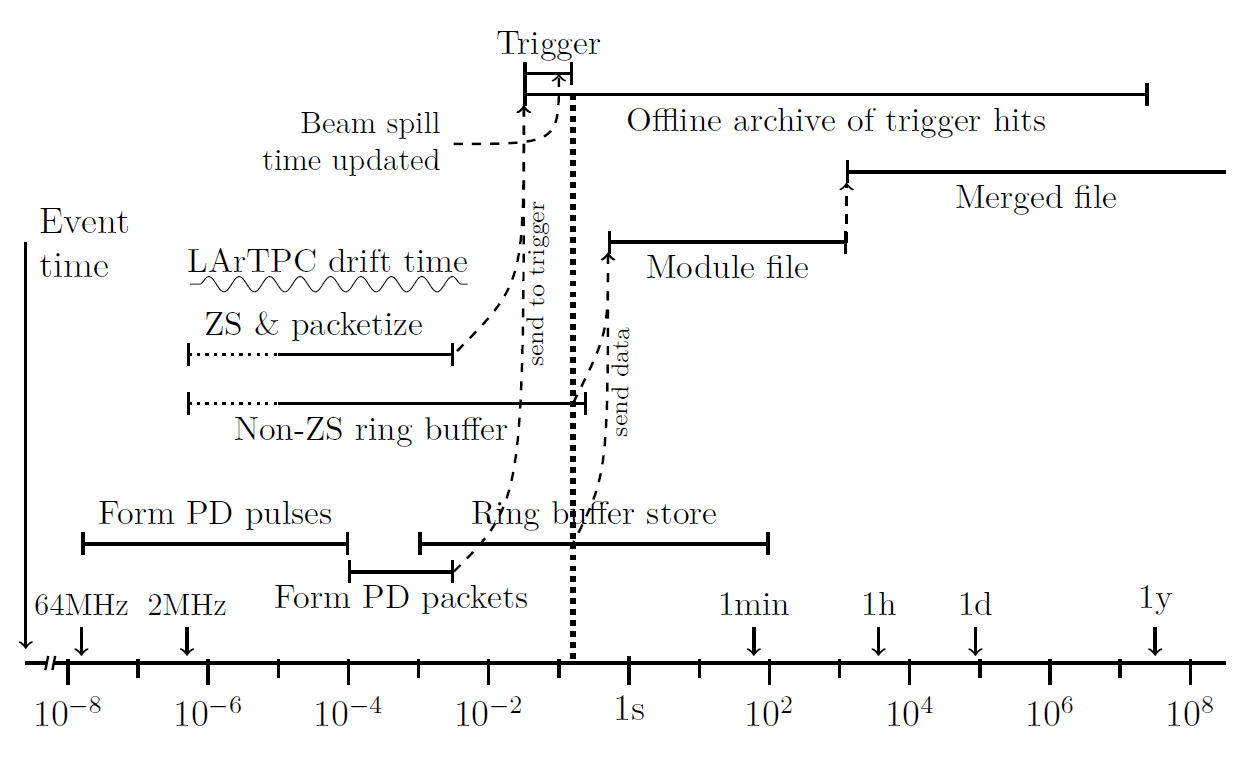
\includegraphics[width=0.8\textwidth]{daq-steps.png}
	\caption{Main DAQ steps displayed relative to the event time.}
	\label{fig:fddaqtime}
\end{figure}

The time sequence, trigger deadlines and buffering of the readout are all
shown in Figure~\ref{fig:fddaqtime}.  This figure shows time in the
horizontal direction on a logarithmic scale to indicate how long after
the particles appear in the detector each process can start and must
finish.  There is one level of triggering, with a trigger deadline
(latest time a trigger decision can arrive) of
0.16\,s after the event has occurred, indicated by the vertical dotted
line.  This is long enough that in 99\% of the cases, a message will
arrive from the Fermilab site to update the predicted time of a
neutrino spill with the actual time in order that the detector can be
triggered independently of any signals in the detector.  This
operation has been used succesfully on MINOS for many years.  

As shown in Figure~\ref{fig:fddaqtime}, prior to the trigger time and
independently in each detector module, the detector readout assembles
packets of data corresponding to fixed time intervals and sends them
to the trigger event builders.  Both the LArTPC readout and the SSP
readout (\ref{sec:pd}) send zero-suppressed data, suitable for triggering, to a set
of event-builder processes that run in parallel, each accepting all
the data from the entire 10-kt module for a specific time interval and
performing trigger algorithms on them.  All time intervals are
processed so that the trigger has no dead time.  The data from the LArTPC and SSP
are also stored in ring buffers
  to await collection after an
affirmative trigger decision --- in the case of the LArTPC, this data
is not zero suppressed.  The data are built into events in a ``10kt-module
file'' that is written to disk.  About an hour later, an offline process merges
the data from the separate 10-kt module files and archives them at the host lab.

To maximize data collection for a supernova, the continuous
zero-suppressed trigger data is kept in a large buffer area on disk.
Ways to collect data that are cropped more gently than the zero-suppressed 
data stream during the extended period of a supernova are
under study: the non-zero-suppressed ring buffers on the current
design of RCEs are sufficient for 0.4\,s of buffering; the trigger farm can send
instructions in the trigger messages to manage storage of data in
these buffers during a supernova. Two possible extensions
are
\begin{itemize}
\item extend the buffer memory , either on the RCEs or elsewhere in the aTCA crate, or

\item use the powerful intercommunications between RCEs to cause neighboring
channels to be kept around the time of a potential supernova event candidate. 

\end{itemize}

%\begin{cdrtable}[Estimated data rates]{lcc}{daqrefrates}{Estimated data  rates in the DAQ system}  %The third argument (reads {cc}) can use c, l, r or p{some length} % but please do %not include lines like “|c|l|l|”. It CAN look like {cll} or {llp{3cm}}, for instance.
%Process & Rate (kHz/APA) & Data rate (MBytes/s) \\ \toprowrule
%Generic 2.3\,ms interval & 0.43 & 6,000\\ \colhline
%Cosmic ray muons (4850L) & $6\times 10^{-7}$ & $1\times 10^{-5}$ \\ \colhline
%Radioactivity & $\sim 64$ & 1.9 \\ \colhline
%Electronics noise (not common mode) & $\sim 1$ & 0.03 \\
%\end{cdrtable}

%At the 4850L, the data rate in the trigger is dominated by
%radioactivity from $^{39}$Ar and $^{85}$Kr.  The cosmic-rays that
%occur about once per minute are the major source of events that should
%be collected on the data stream; the physics beam events, atmospheric
%netrinos and other candidate contained events are included in this data budget.  
%Table~\ref{tab:daqrefrates}) gives estimates of the
%rate of occurence of these events and the expected ``steady-state'' data rate
%(after the derandomisation provided by the buffering in the front-end
%computers).

The requirements for handling radiological and other backgrounds (e.g. $^{39}$Ar decays as described
in~\ref{sec:ar39decays}) are met in this conceptual design by the very high throughput provided by modern
off-the-shelf components  and the parallelism provided by artDAQ, which makes the design extendable to avoid bottolenecks.  The triggering
allows the zero-suppression to be tuned to optimise for the final
level of noise, while retaining the maximum level of information for
the important physics events.

%This DAQ design is being prototyped for the 35t tests in 2015, with
%two COBs (containing 16 RCEs) and eight SSPs.  The artDAQ software
%toolkit is being used to implement the readout, event-building and
%triggering, although we are not implementing the ``collect-twice''
%model for the 35t.

